\section{Camera and image formation process}
\label{imageFormation}

To understand how a camera perceives the environment, it is necessary we understand the image formation process. For us humans, we “see” things when a light originating from a light source is reflected on an object and enters our eyes. A camera acts very much similar to the human eye. The earliest and first model of an optical camera is the pinhole camera which is a simple and highly accurate representation of our eye model. This is the simplest device to form an image of a 3D scene on a 2D surface. As seen in figure 1 rays of light enter the pinhole and forms an inverted image of the object. This is called perspective projection. As the image formed in the image place is inverted, we consider a virtual plane in front of the pinhole that acts as the image plane.  

% For one-column wide figures use
\begin{figure}[H]
% Use the relevant command to insert your figure file.
% For example, with the graphicx package use
  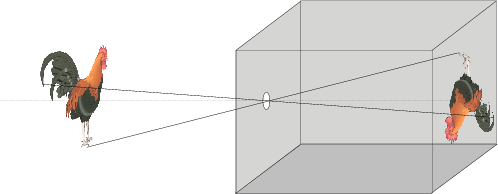
\includegraphics[width=\textwidth]{./figures/imageFormation.png}
% figure caption is below the figure
\caption{Pinhole Image formation}
\label{fig:1}       % Give a unique label
\end{figure}

Although the pinhole model is quite accurate, modern cameras have lenses. They help gather more light from a source leading to higher quality sharper images. Ignoring the internal diffraction, we assume thin lens equations for the imaging process. Every camera has a region of depths over which the scene is sharp. Modern cameras have variable apertures which help in focusing on objects at varying distances in the scene.  

Every camera has an intrinsic, extrinsic and distortion parameters that are important to understand for every application. These parameters are used to correct for lens distortion, measure objects in physical world and to determine the location of the camera in the real world. Camera calibration is the process of estimating these parameters specific to a given camera and application setup. Figure 2 demonstrates how the a real world 3D coordinate is related to a 2D pixel coordinate using the parameters mentioned above.

The intrinsic camera matrix \textbf{K} is given by
\begin{equation}
K = 
\begin{pmatrix}
  f_x & s & c_x \\
  0 & f_y & c_y \\
  0 & 0 & 1 \\
 \end{pmatrix}
\end{equation}
where $(f_x, f_y)$ is the focal length, $(c_x, c_y)$ is the optical center
and $s$ is skew factor.

The extrinsic camera matrix $\textbf{[R|t]}$ is given by
\begin{equation}
R = 
\begin{pmatrix}
  r_1 & r_2 & r_3 \\
  r_4 & r_5 & r_6 \\
  r_7 & r_8 & r_9 \\
 \end{pmatrix}
t = 
\begin{pmatrix}
  t_x \\
  t_y \\
  t_z \\
 \end{pmatrix}
\end{equation}
where $R$ is the rotation matrix and $t$ is the translation vector between the camera center and world co-ordinates. 

The camera matrix $P$ is given by 
\begin{equation}
P = K[R t]
\end{equation}

% For one-column wide figures use
\begin{figure}[H]
% Use the relevant command to insert your figure file.
% For example, with the graphicx package use
  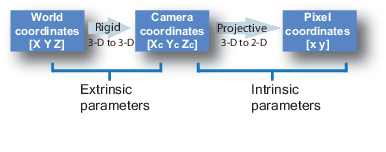
\includegraphics[width=\textwidth]{./figures/imageParams.png}
% figure caption is below the figure
\caption{Camera calibration}
\label{fig:2}       % Give a unique label
\end{figure}

The extrinsic parameters relate the rotation R and translation t of the camera origin at the optical center to the world frame. The intrinsic parameters consists of the focal length given by fx and fy, the optical center given by cx and cy and the skew coefficient s. The distortion parameters consists of radial and tangential distortion along the x and y direction respectively. The number of coefficients are decided based on the lense in consideration. Camera calibration techniques presented in [4] [5] and [6] are widely used in commercial and open source camera calibration tool boxes.